\documentclass{article}
\usepackage[utf8]{inputenc} %Input encoding

\usepackage{amsmath} %Extra math symbols and operators
\usepackage{amssymb}
\usepackage{amsthm}
\usepackage{eufrak}

\usepackage{float}

\usepackage{bm} %Bold symbols

\usepackage{graphicx} %Images

\usepackage{tikz-cd} %Diagrams

\usepackage{enumitem} %Enumerate Labels

\usepackage[margin=1.5in]{geometry} %Adjust Margins

\usepackage{siunitx} % easily format numbers with dimensions
\usepackage{hyperref}
\usepackage{cleveref}
\usepackage{todonotes}

%\usepackage{fancyhdr} %Name on every page
%\pagestyle{fancy}
%\lhead{Rune Buckinx}

\usepackage{mdframed}
\newmdtheoremenv{definition}{Definition}[section]
\newmdtheoremenv{question}{Question}[section]
\newmdtheoremenv{lemma}{Lemma}[section]
\newmdtheoremenv{proposition}{Proposition}[section]
\newtheorem{example}{Example}[section]
\newtheorem{remark}{Remark}[section]
\newmdtheoremenv{theorem}{Theorem}[section]
\newmdtheoremenv{exercise}{Exercise}

\usepackage{import}
\usepackage{xifthen}
\usepackage{pdfpages}
\usepackage{transparent}

\newcommand{\incfig}[1]{
    \def\svgwidth{\columnwidth}
    \import{./figures/}{#1.pdf_tex}
}

\usepackage[backend=biber]{biblatex}
\addbibresource{references.bib}
%\tikzset{component/.style={draw,thick,circle,fill=white,minimum size =0.75cm,inner sep=0pt}}

\title{Modeling of MHD waves in the solar corona}
\author{Micha\"el Maex \and Rune Buckinx}
\date{March 2020}

\begin{document}

\maketitle

\begin{abstract}
    This paper presents a summary of research for a bachelor's thesis on the modelling of magnetohydrodynamic waves in the solar corona using numerical simulations via the open source code PLUTO. 
\end{abstract}
\tableofcontents

\listoftodos

\newpage
\section{Introduction} \label{sec:introduction}
The Sun's corona, or solar corona, is the outer layer of the Sun's atmosphere, which consists of fully ionized material due to it having very high temperatures compared to the surface of the sun. 
As the particles of this fluid are charged the fluid interact with the magnetic field and electric currents in the fluid have to be taken into account.  
The plasma in the solar corona can be described using magnetohydrodynamic (MHD) equations, which combine the Navier-Stokes equations from fluid dynamics with the Maxwell equations from electromagnetism. 
This approach to model the plasma treats it as a single fluid, as opposed to the two-fluid model, which describes the ions and electrons seperately. \\

The differential/governing equations that make up the MHD model, are difficult to solve analytically. 
It is therefore favourable to use numerical computer modelling to study the equations, which is the main focus of this bachelor's project. 
The simulations will be performed in the open source code PLUTO, which is designed to solve systems of partial differential equations in astrophysical fluid dynamics \cite{mignone2011pluto}. 

\section{(M)HD Theory} \label{sec:(m)hd_theory}

\subsection{Magnetohydrodynamics and the solar corona} \label{sec:magnetohydrodynamics_and_the_solar_corona}
The classic Navier-Stokes equations do not suffice to describe the movement in the solar corona due to the influence of strong magnetic fields on the ionized particles. This magnetic field stems from convection in the photosphere, which is a physical process that helps transport the nuclear energy created in the core of the sun \cite{brun2017magnetism}.\\

The use of the magnetohydrodynamic model to describe the plasma depends on three main assumptions, namely, high collisionality, large scales and the assumption of ideal fluids. The last assumption implies that the dissipation of large scale variables is neglected \cite{goedbloed2004principles}. This model also does not take relativity into account, as opposed to the relativistic magnetohydrodynamic model, which will not be discussed further \footnote{More information about the relativistic MHD model can be found in \cite{karas2005introduction}}.

Magnetohydrodynamics can be described by a system of partial differential equations. 
Just like ordinary fluid dynamics, these are derived from conservation laws. 
In this report we will only consider the non-relativistic approximation. \todo{remove redundant information} 
The system of PDE's/conservations laws is the following:
\begin{alignat}{3}
    &\frac{\partial \rho}{\partial t} &&+ \nabla \cdot (\rho \mathbf v) &&= 0 \tag{mass}\label{masscont}\\
    &\frac{\partial \mathbf m}{\partial t} &&+  \nabla \cdot \bigg[\mathbf{mv - BB+ I}\bigg(p + \frac{\mathbf B^2}{2}\bigg)\bigg]^T &&= -\rho \nabla \Phi \tag{moment}\label{cauchymoment}\\
    &\frac{\partial \mathbf B}{\partial t} &&+ \nabla \times (cE) &&= 0 \tag{charge}\label{Faraday}\\
    &\frac{\partial(E_t + \rho \Phi)}{\partial t} &&+ \nabla \cdot \bigg[\bigg(\frac{\rho \mathbf v^2}{2} + \rho e + p + \rho \Phi\bigg)v + c \mathbf E \times \mathbf B\bigg] &&= 0 \tag{energy}\label{energy}.
\end{alignat} \todo{Maybe start with the same system of equations as in \cite{FitzpatricknoteS}}.
Here $\rho$ is the plasma density, $\mathbf B$ is the magnetic field,  $\mathbf v$ the velocity, $\mathbf m= \rho \mathbf v$ the momentum density,$\Phi$ the potential, $p$ is the thermal pressure, $E_t$ is the total energy, which is given by \[
E_t, = \rho e \frac{m^2}{2\rho} + \frac{B^2}{2}
.\]  
The constants  $e, c$ are the elementary charge and the speed of light respectively.

If the environment is one where the thermal pressure and density are small deviations of some constant background pressure and density, $p_0, \rho_0$. Then the speed of sound is given by \[
c_s^2 = \gamma \frac{p_0}{\rho_0}
,\]
where $\gamma = \frac{f + 2}{f}, $ with $f$ the degrees of freedom of a particle. In a plasma $f$ is almost always $3$. 

\section{Linear Approximations} \label{sec:linear_approximations}

To analyse small amplitude waves in the plasma, a linearised version of the magnetohydrodynamic equations is considered as in \cite{Fitzpatricknotes}, namely

\begin{alignat}{3}
    &\frac{\partial \rho_1}{\partial t} &&+ \nabla \rho_0 \cdot (\mathbf v_1) &&= 0 \tag{mass}\label{masslin}\\
    \rho_0&\frac{\partial \mathbf v_1}{\partial t} &&+  \nabla p_1 - \frac{(\nabla \times \mathbf{B_1}) \times \mathbf{B_0}}{\mu} &&= 0 \tag{moment}\label{cauchymomentlin}\\
    &\frac{\partial \mathbf B_1}{\partial t} &&+ \nabla \times (\mathbf{v_1} \times \mathbf{B_0}) &&= 0 \tag{charge}\label{Faradaylin}\\
    &\frac{\partial}{\partial t}(\frac{p_1}{p_0} - \frac{\gamma\rho_1}{\rho_0}) && &&= 0 \tag{energy}\label{energylin}.
\end{alignat}

Where $\mu$ is the vacuum permeability constant, and initial flow velocity and plasma current are assumed to be zero. This linearisation is done by writing the physical quantities as
\begin{equation*}
    f(\mathbf{x},t) = f_0(\mathbf{x}) + f_1(\mathbf{x},t)
\end{equation*}
under the assumption that the perturbation ($f_1$) of the equilibrium ($f_0$) is small compared to this equilibrium.
The further analysis is based on the online lecture notes by R. Fitzpatrick \cite{Fitzpatricknotes}.\\

Consider perturbations of the following form, $\exp(i(\mathbf{kx} + \omega t))$, substituting this in the equations results in the following system of equations,

\begin{alignat}{3}
    &-\omega\rho_1 &&+  \rho_0 \mathbf{k}\cdot\mathbf v_1 &&= 0 \\
    &-\omega\rho_0\mathbf v_1 &&+  \mathbf{k} p_1 - \frac{(\mathbf{k} \times \mathbf{B_1}) \times \mathbf{B_0}}{\mu} &&= 0 \\
    &-\omega\mathbf B_1&&+ \mathbf{k} \times (\mathbf{v_1} \times \mathbf{B_0}) &&= 0 \\
    &-\omega(\frac{p_1}{p_0} - \frac{\gamma\rho_1}{\rho_0}) && &&= 0 .
\end{alignat}

Rewriting these equations in function of the equilibrium states and $\mathbf{v_1}, \mathbf{k}$ and $\omega$ leads to,
\begin{align*}
    \rho_1 &= \rho_0 \frac{\mathbf{k} \cdot \mathbf{v_1}}{\omega}\\
    p_1 &= \gamma p_0 \frac{\mathbf{k} \cdot \mathbf{v_1}}{\omega}\\
    \mathbf{B_1} &= \frac{(\mathbf{k} \cdot \mathbf{v_1}) \cdot \mathbf{B_0} - (\mathbf{k} \cdot \mathbf{B_0})\cdot \mathbf{v_1}}{\omega}
\end{align*}
These values can now be subsituted in the linearised moment equation yielding the following,
\begin{equation*}
    -\omega\rho_0\mathbf{v_1} + \mathbf{k}\cdot \frac{\gamma p_0}{\omega}-\frac{(k\times \frac{(\mathbf{k} \cdot \mathbf{v_1}) \cdot \mathbf{B_0} - (\mathbf{k} \cdot \mathbf{B_0})\cdot \mathbf{v_1}}{\omega})\times \mathbf{B_0}}{\mu} = 0
\end{equation*}
Further rearranging of the terms gives,
\begin{equation}
    \bigg(\omega^2 - \frac{(\mathbf{k \cdot B_0)^2}}{\mu\rho_0}\bigg)\mathbf{v_1} = \bigg[\bigg(\frac{\gamma p_0}{\rho_0}- \frac{\mathbf{B_0}^2}{\mu\rho_0}\bigg)\mathbf{k} - \frac{(\mathbf{k \cdot B_0)}}{\mu\rho_0}\mathbf{B_0}\bigg](\mathbf{k\cdot v_1}) - \frac{(\mathbf{k \cdot B_0})(v_1\cdot B_0)}{\mu\rho_0}\mathbf{k}
\end{equation}
To simplify further notation, $c_s = \sqrt{\frac{\gamma p_0}{\rho_0}}$ will be used to represent the sound speed, and $v_A = \sqrt{\frac{\mathbf{B_0}^2}{\mu\rho_0}}$ will be used to represent the ``Alfv\'en speed''. Under the assumption that the magnetic field lies in the $x$-direction, and the wave front vector $k$ lies in the $x,y$-plane this can be rewritten as follows, where $\theta$ represents the angle between $\mathbf{B_0}$ and $\mathbf{k}$.
\begin{equation*}
\begin{pmatrix}
\omega^2 - \mathbf{k}^2c_s^2 - \mathbf{k}^2v_A^2 & - \mathbf{k}^2c_s^2& 0\\
? & ? & 0\\
0 & 0 & ?
\end{pmatrix}
\begin{pmatrix}
v_x \\
v_y \\
v_z
\end{pmatrix}
=
\begin{pmatrix}
0\\
0\\
0
\end{pmatrix}
\end{equation*}
\subsection{Alfv\'en Waves}
The previous derivation led to two different types of waves, namely, Alfv\'en waves and sound waves. An Alfv\'en wave is a magnetic tension wave caused by a restoring force. 
This force follows from Lenz's law, which states that the electrical currents caused by the motion of a conducting fluid in a magnetic field give rise to a force countering this motion, and Newton's second law for fluids \cite{Finlay2007}. 
Properties of Alfv\'en waves are that they travel along the magnetic field lines and hence cannot propagate across field lines and that they do not perturb density \cite{mhdppt}.\\



\section{Pluto Code} \label{sec:pluto_code}

\todo{Hier zou ik iets schrijven over hoe pluto werkt}

\subsection{Units in Pluto} \label{sec:units_in_pluto}

Internally Pluto uses dimensionless code units. All units are derived from the constants \texttt{UNIT\_DENSITY} ($\rho_0$), \texttt{UNIT\_LENGTH} ($L_0$), \texttt{UNIT\_VELOCITY} ($v_0$), all of which are denoted in cgs units. All other units are derived from these units.  
Note that the unit for magnetic field is defined as $B_0 = v_0\sqrt{4\pi \rho_0} $.

\Cref{tab:default_units} shows some important dimensions in (M)HD and what one code unit represents when \texttt{UNIT\_DENSITY}, \texttt{UNIT\_LENGTH} and  \texttt{UNIT\_VELOCITY} have their default values.
\begin{table}[htpb]
	\centering
	\caption{Important dimensions and their code units in PLUTO}
	\label{tab:default_units}
	\begin{tabular}{c|c}
		one code unit of & corresponds to\\
		\hline 
		density & $m_p$ \si{\per \centi\metre\cubed} = \SI{1.67262171e-24}{\gram \per \centi\metre\cubed}\\
		lenth &\SI{1}{AU} \\
		velocity & \SI{1}{\kilo\metre \per \second}\\
		time & \SI{149597892}{\second} \\
		magnetic field strength & \SI{4.584624773e-07}{Gs} \\
		pressure & \SI{1.67262171e-14}{Ba} = \SI{1.6726217e-15}{Pa}
	\end{tabular}
\end{table}

\subsection{Initial example} \label{sec:initial_example}
The first problem that will be analysed is a simple hydrodynamic blastwave generated by a high-pressure region. 
The viscosity, heat conduction and dissipation of the fluid will be neglected. 
This problem is meant to be an initial example of how to set up a non-predefined simulation and is a modified version of the initial example described in section 0.4 of PLUTO's User Guide \cite{plutouserguide}. 
The blastwave is simulated in two dimensions and uses three user-defined parameters, namely, the ambient pressure, the pressure in the high-pressure region, and $\gamma$ which in this report will always be $5/3$. 
The domain is a rectangle goin from -10 to 10 (code units), in both the $x$ and the $y$ direction, wich is represented by a $1024\times 1024$ grid. 

The following initial condition is used, a high-pressure region inside a circle of radius 0.3 is surrounded by an ambient pressure region. The simulation is run for X units of time, and every Y units, a double-precision file is saved.\\

PLUTO's hydrodynamics module solves the following system of equations

\begin{alignat}{3}
    &\frac{\partial \rho}{\partial t} &&+ \nabla \cdot (\rho \mathbf v) &&= 0 \tag{mass}\label{masscont}\\
    &\frac{\partial \mathbf m}{\partial t} &&+  \nabla \cdot (\mathbf{mv + I}p)^T &&= -\rho \nabla \Phi \tag{moment}\label{cauchymoment}\\
    &\frac{\partial(E_t + \rho \Phi)}{\partial t} &&+ \nabla \cdot ((E_t + p +\rho\mathbf{\Phi})\mathbf{v}) &&= 0 \tag{energy}\label{energy}.
\end{alignat}

These can be derived from the standard Euler equations by changing the total derivatives to partial derivatives with respect to time. This is necessary because PLUTO uses a static grid to run simulations, and hence uses local change. \todo{Hier nog nodig om die afleiding bij te zetten?}
\begin{figure}[h]
	\centering
	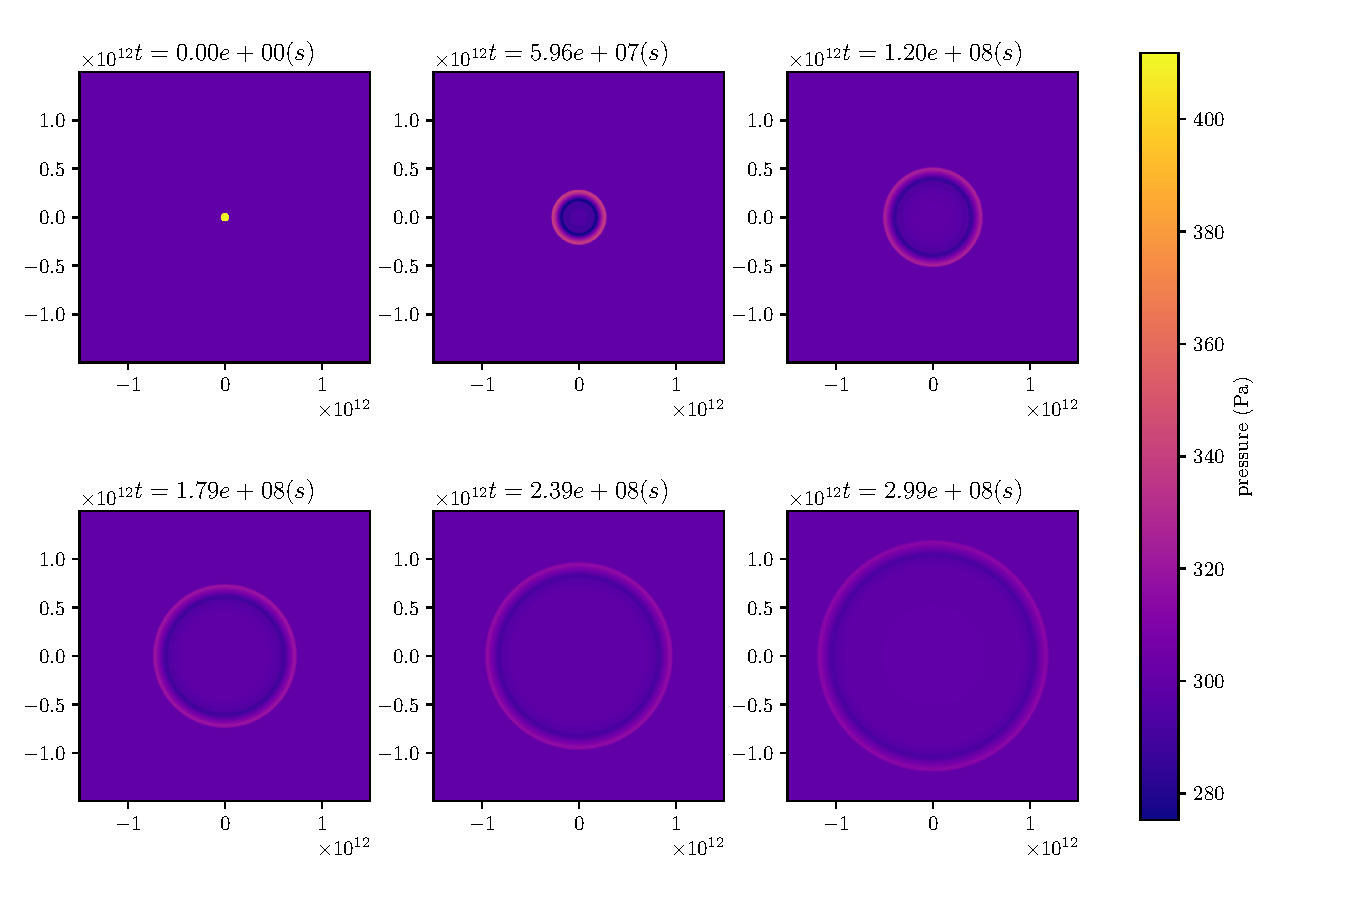
\includegraphics[width=\textwidth]{figures/blast_wave.pdf}
	\caption{propagation of a blastwave in the absence of a magnetic field}
	\label{fig:blastwave}
\end{figure}

\Cref{fig:blastwave} shows pressure of the simulated fluid at multiple points in time. 
The speed at which the wave front moves is the group speed. 
According to \cref{sec:magnetohydrodynamics_and_the_solar_corona} this is given by $c_s = \sqrt{\frac{5}{3} \frac{p_0}{\rho_0}} $. Hence the speed (in code units) is $\sqrt{\frac{5}{3}8} = 3.61$, which corresponds to \SI{3.61e5}{\centi\metre\per\second}.
A comparison of the theoretical radius against the simulated radius can be found in \cref{fig:wave_front_speed}. 
Note that the curve of the simulation is jagged because the grid on which the simulation is run is discreet. 
Initially the simulated wave moves faster than the theoretical group speed. 
This could be an result of the linear approximation used in determining the group speed.
However for the remainder of the simulation the wave front matches the theoretical group speed quite well.


\begin{figure}[h]
	\centering
	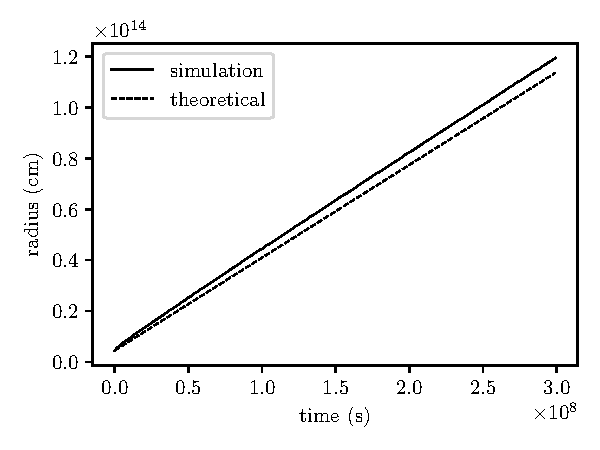
\includegraphics[width=0.6\textwidth]{figures/wavefront_position}
	\caption{The position of the simulated wave front compared to the theoretical speed}
	\label{fig:wave_front_speed}
\end{figure}

\subsection{Non-linear effects} \label{sec:nonlinear_effects}
Due to our current understanding of the (magnetic) navier-stokes equations, linear approximations are necessary for many theoretical results. 
This is one limitations of the theory that numerical simulations aim to solve.
A problem was setup with the same initial conditions as in \cref{sec:initial_example}, except that the initial pressure is 100 (code units) in the centre and 8 elsewhere. 
Like in the previous setup the radius of the blast over time was compared to the theoretically linear group speed.
\Cref{fig:non_linear_effects} shows concave radius/time relation against the linear theoretically predicted relation. 
\begin{figure}[h]
	\centering
	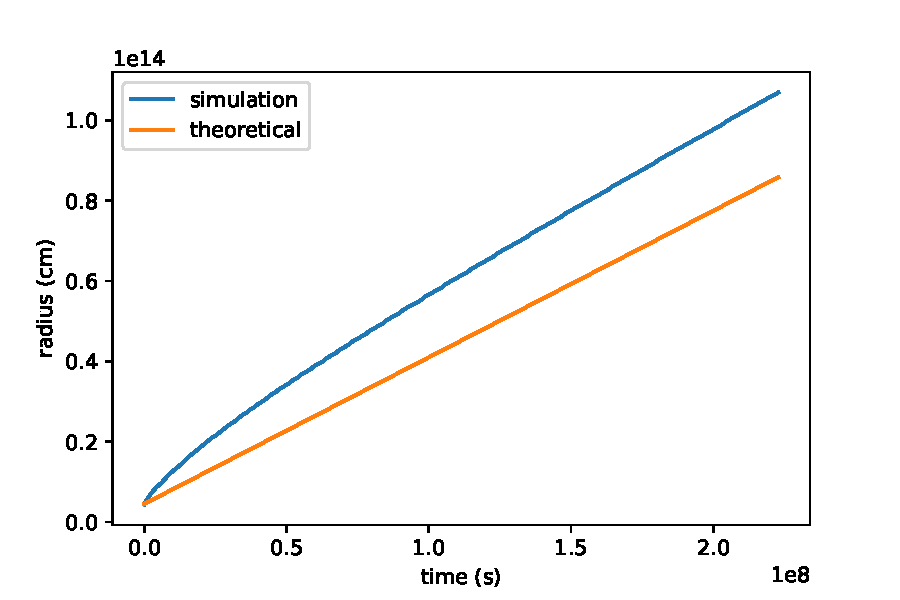
\includegraphics[width=0.6\textwidth]{figures/non_linear_effects.pdf}
	\caption{A comparison of the theoretically predicted radius of the blast wave (using a linear approximation) versus the simulated result}
	\label{fig:non_linear_effects}
\end{figure}

\section{Waves in magnetohydrodynamic fluids} \label{sec:waves_in_magnetorhydrodynamic_fluids}
In order to study the effects of a constant magnetic background field, the same initial conditions as in \cref{sec:initial_example} were used but this time a magnetic field in the $x$ direction was added.
The parameter $\beta = \frac{2p}{B^2}$ (in code units) gives the ratio of magnetic pressure over mechanical pressure. 
If $\beta = \infty$ the magnetic field is $0$. 
If $\beta \ll 1$ the magnetic pressure dominates. 
\Cref{fig:blastwave_shape_beta} shows how the value of $\beta$ influences the shape of the blast wave.
\todo{Add what is plotted to figures (pressure)}
\begin{figure}[H]
	\centering
	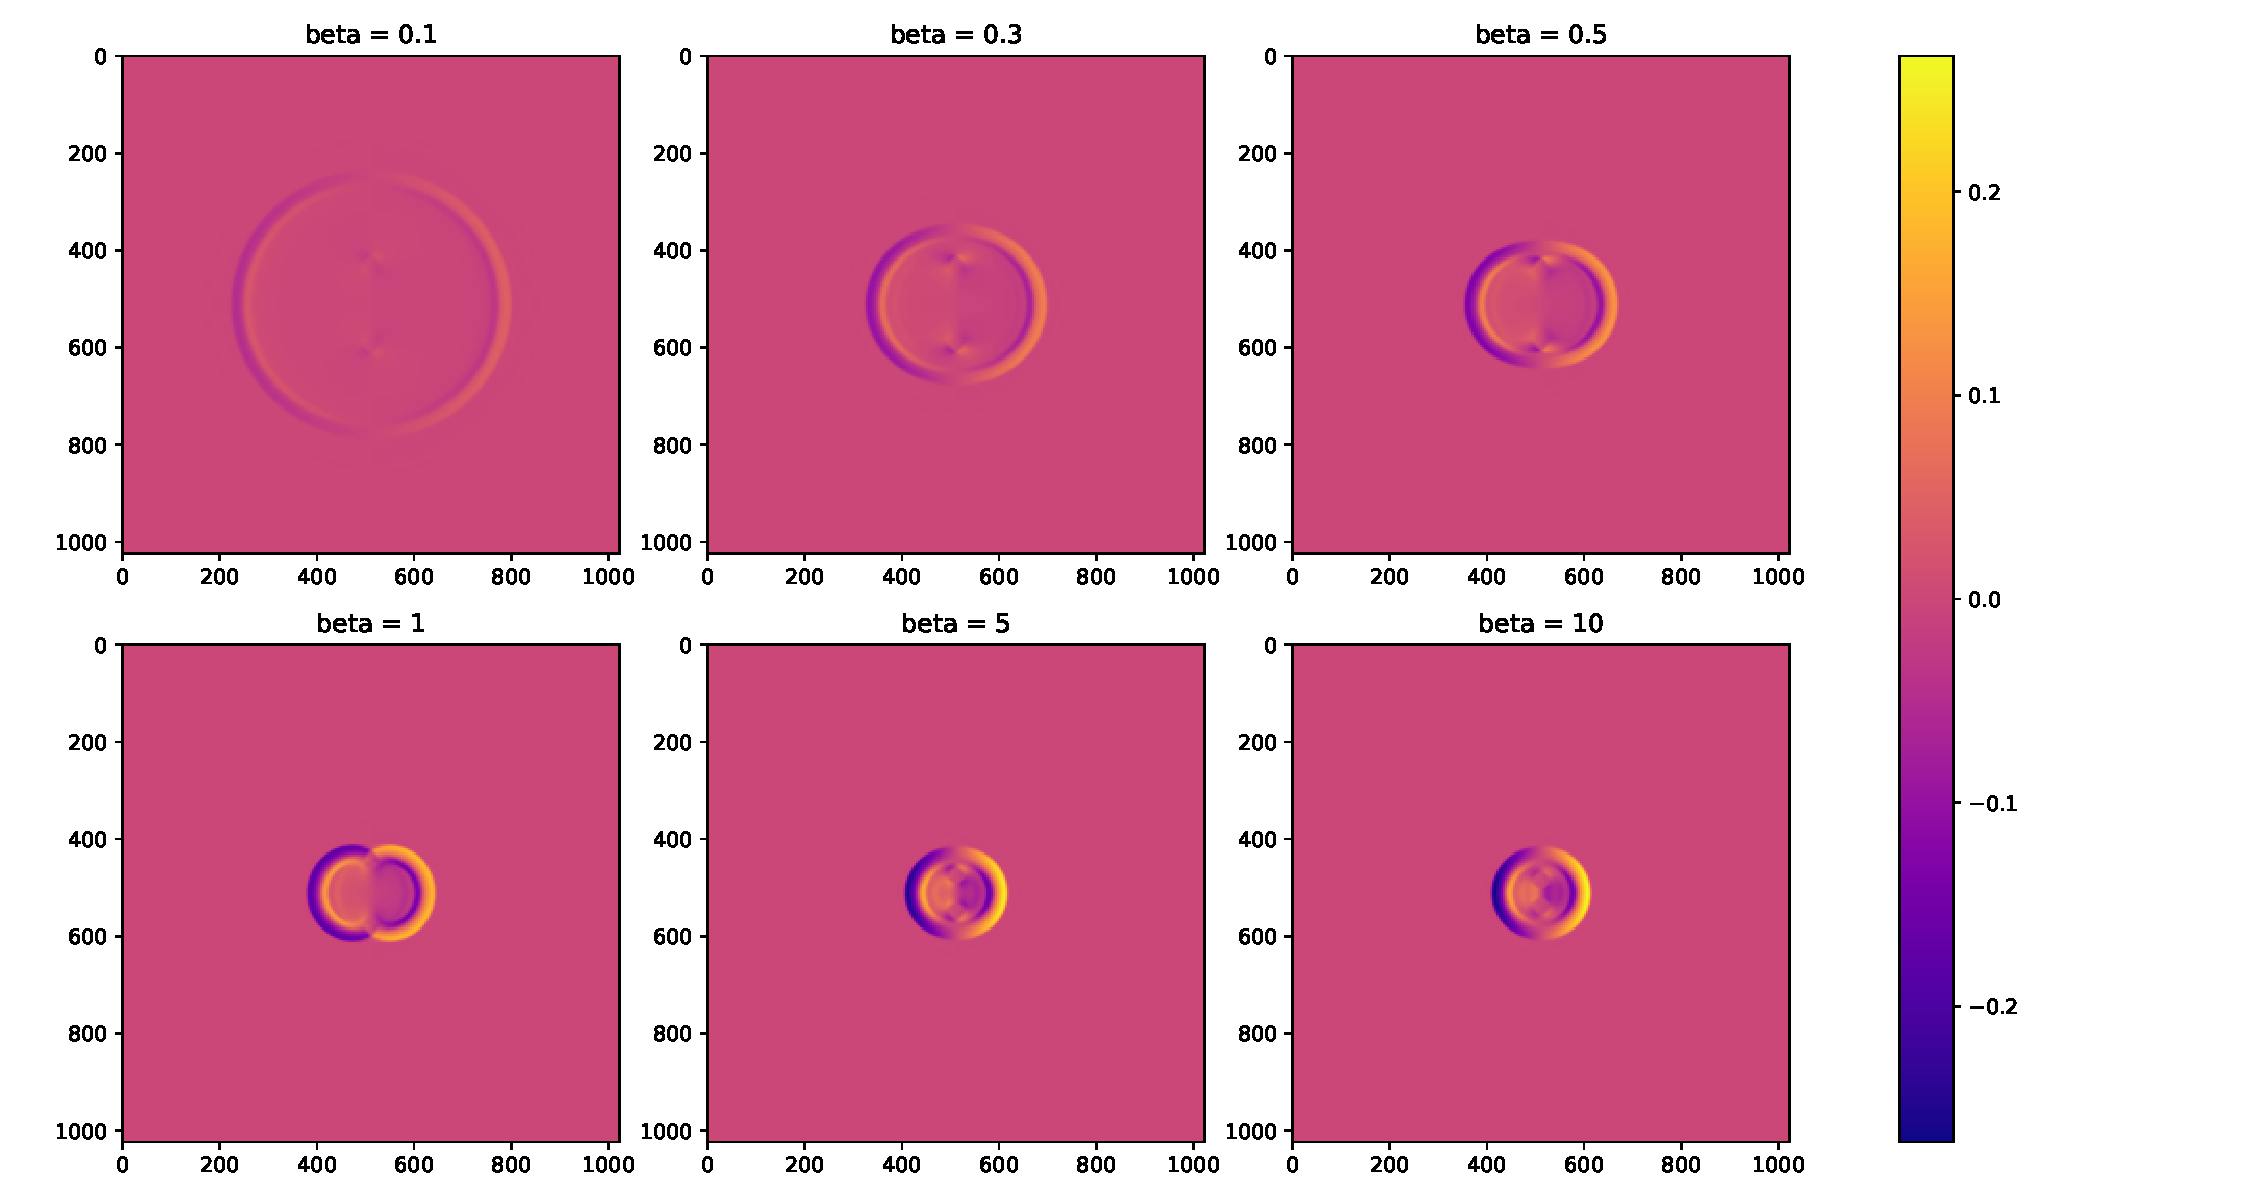
\includegraphics[width = \linewidth]{figures/influence_beta.pdf}
	\caption{The shape of the blast wave for different plasma beta's.}
\label{fig:blastwave_shape_beta}
\end{figure}

When $\beta  = 10$ the magnetic pressure is dominant the alfv\'en \todo{This is not an alv\'en wave} waves are clearly visible.

\todo{comparison sound speed theoretical vs simulation}
\begin{figure}[H]
	\centering
	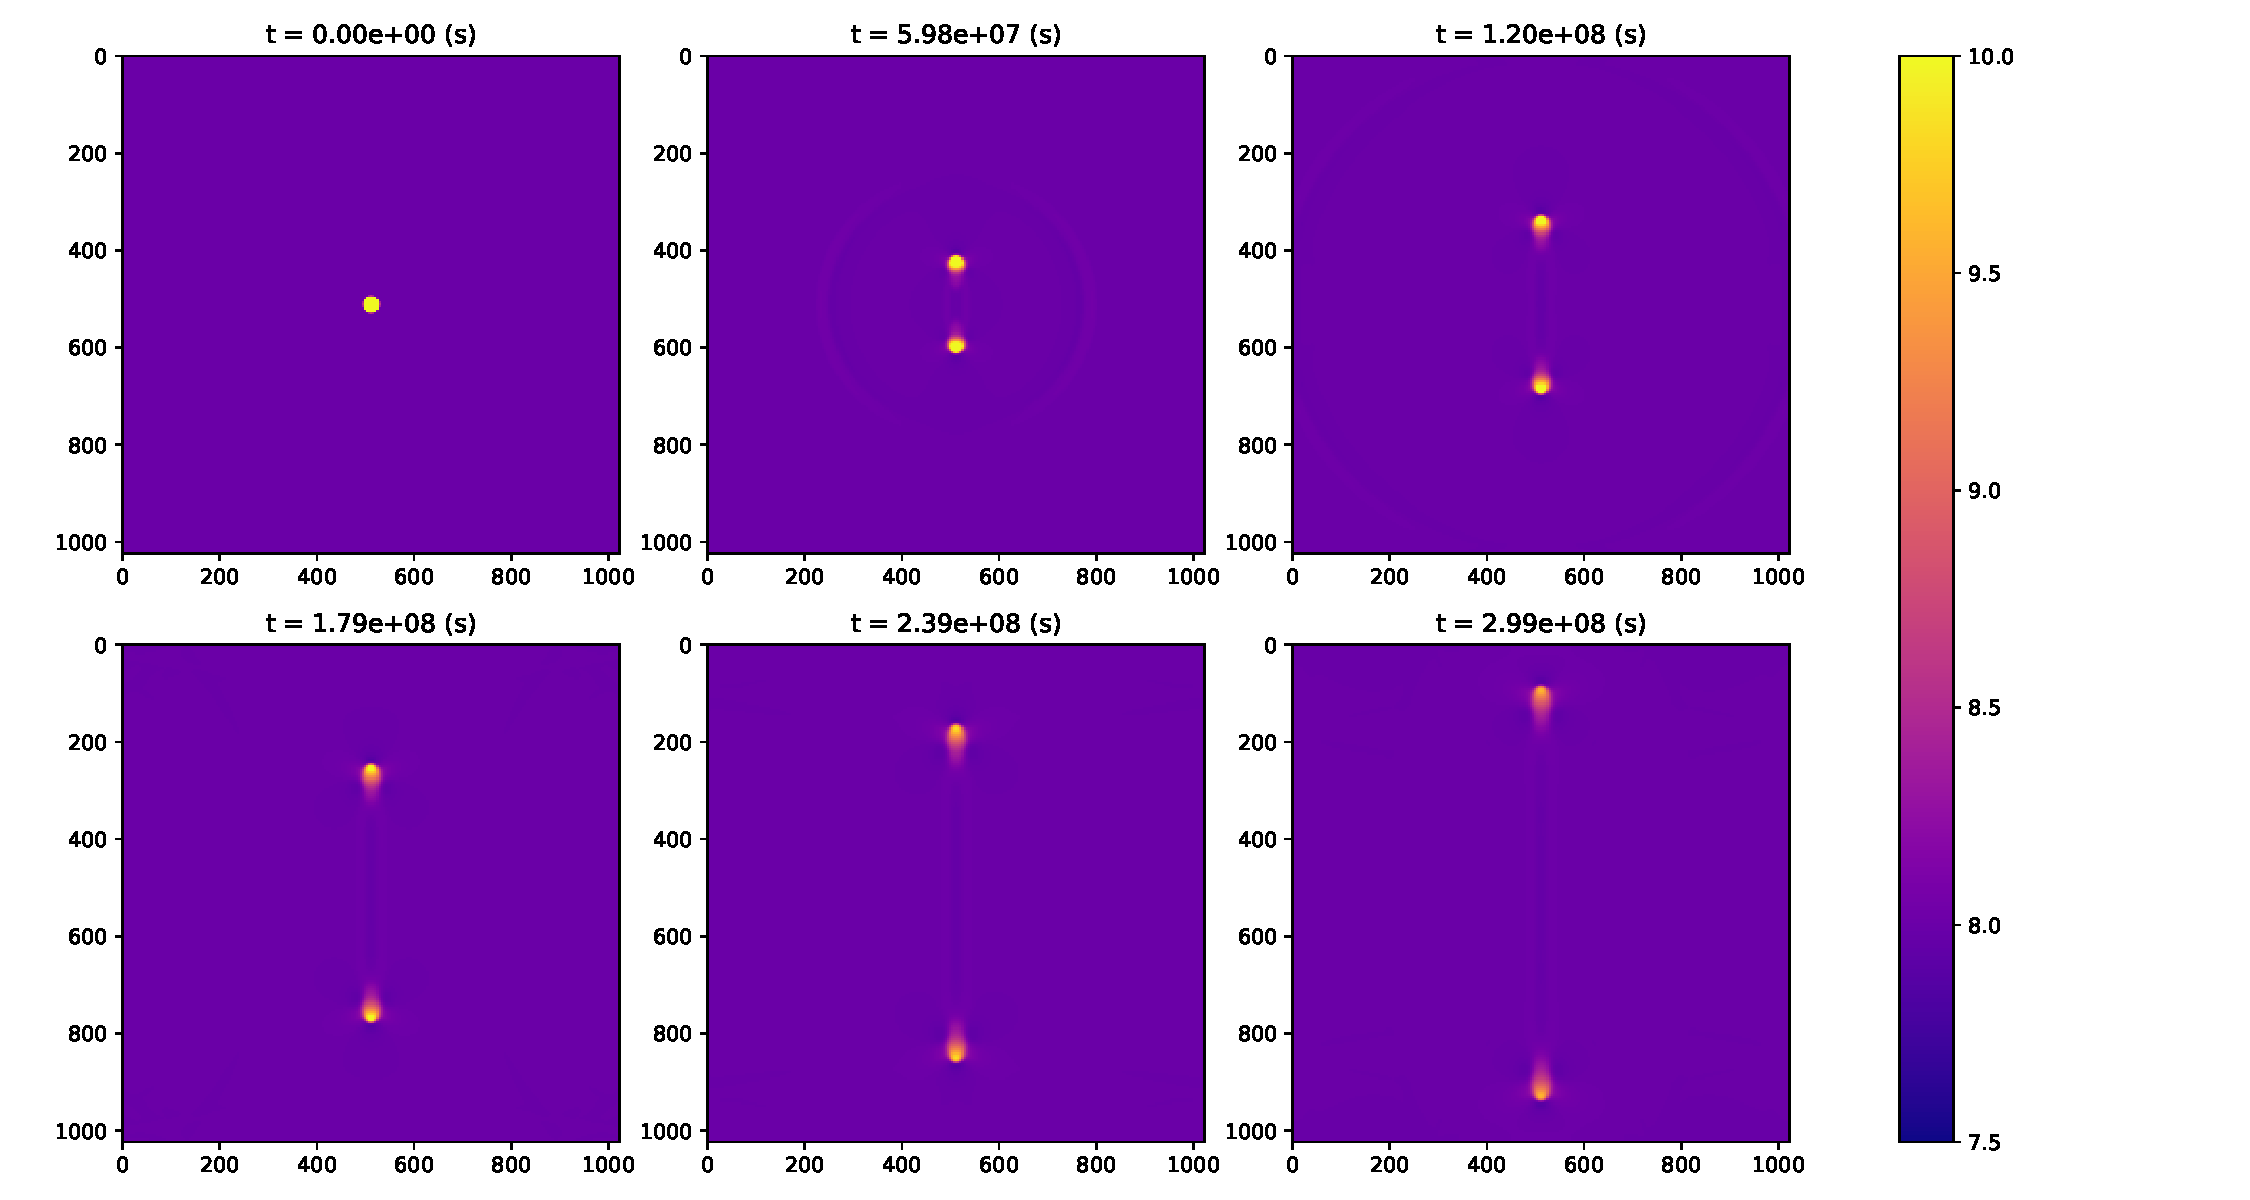
\includegraphics[width=\textwidth]{figures/alven_wave.pdf}
	\caption{}
	\label{fig:Alfven_wave}
\end{figure}
\todo{Derivation of sound wave speed and Alfven Wave speed}

In the simulation above \cref{fig:Alfven_wave}, the magnetic field lies in the $x$-direction, hence the Alfv\'en wave is a one-dimensional wave, also in the $x$-direction. 
The theoretical speed of this wave is $v_A = \frac{B_0}{\sqrt{\rho_0}} = \sqrt{\frac{\beta p_0}{\rho_0}} = 8.94$ in code units. 
This corresponds to a physical speed of \SI{8.94e5}{\centi\meter\per\second}.
\Cref{fig:alven_wave_speed} compares this to the propagation of the waves tops in the simulation.
\begin{figure}[H]
	\centering
	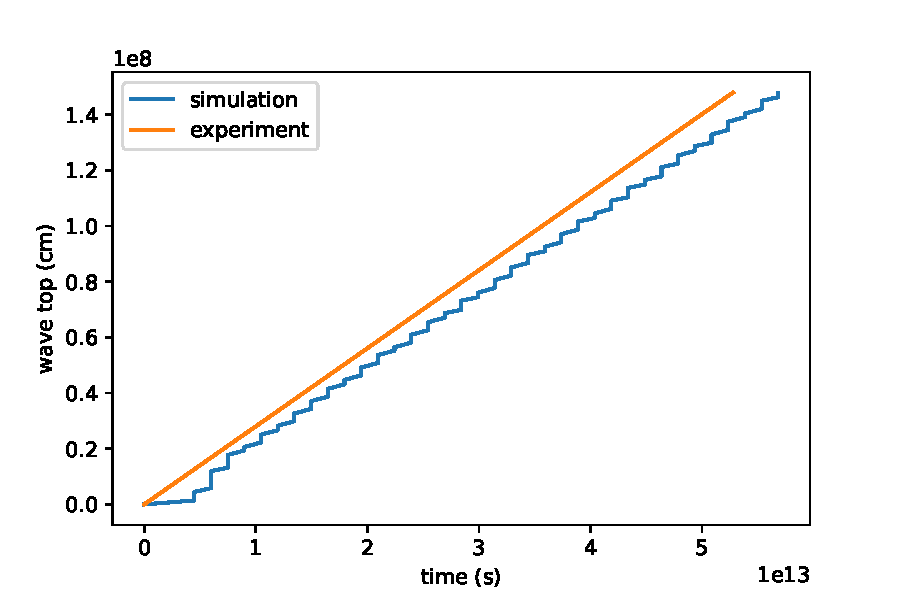
\includegraphics[width=.6\textwidth]{figures/alven_wave_position.pdf}
	\caption{The position of the wave top of the Alfv\'en wave compared to the theoretical speed.}
	\label{fig:alven_wave_speed}
\end{figure}
\todo{Change text in figure experiment -> theoretical}
\todo{Compare Alfven wave speed theoretical and empirical}
\subsection{Sound Waves}
\section{Interaction of MHD waves with large scale structures}
This task focuses on the interaction of large scale structures in the solar corona with magnetohydrodynamic waves and is based on the paper titled "Propagation of a global coronal wave and its interaction with large-scale coronal magnetic structures" by Afanasyev and Zhukov.  \cite{afanasyev2018propagation}\\

The shock wave simulated in \cref{sec:waves_in_magnetorhydrodynamic_fluids} is a good description of a wave in a uniform plasma, however it does not account for various large scale non-uniformities, such as coronal holes and plumes. The interaction of coronal waves with these structures results in wave phenomena such as wave transmission and reflection, which have been observed in extreme ultraviolet images of the Sun (see for example \cite{gopalswamy2009euv}).
\subsection{Coronal Hole Model}
A coronal hole, is a region of lower temperature and density compared to the surrounding plasma. This results in a region of higher Alfv\'en speed. They occur when a magnetic field does not fall back, and is open to interplanetary space \todo{Degelijke bron nodig}.\\

To simulate a coronal hole, the following initial conditions are used,
\begin{align*}
    n &= n_{\text{out}} - (n_{\text{out}}-n_{\text{in}})\exp\bigg[-\bigg(\frac{r}{d}\bigg)^8\bigg]\\
    T &= T_{\text{out}} - (T_{\text{out}}-T_{\text{in}})\exp\bigg[-\bigg(\frac{r}{d}\bigg)^8\bigg]
\end{align*}
Here $n$ denotes the plasma number density, $T$ denotes the temperature, and $r$ is the distance from the center. The parameter $d$ is used to describe the characteristic size of the non-uniformity and can hence be used to adjust the simulation to the correct order of magnitude. In this simulation $d$ will be equal to $150$ Mm (see also \cref{tab:coronal_hole}).\\

The magnetic field in the simulation is directed in the $z$-direction while the simulation takes place in the $x,y$-plane. An initial equilibrium is achieved by keeping the total pressure constant, using the following equation,
\begin{equation*}
    p^t = p_{\text{gas}} + \frac{B^2}{8\pi} = \text{constant}.
\end{equation*}
Here $p^t$ represents the total pressure, which is the sum of the gas pressure and the magnetic pressure. \\

The values that are used for the parameters are summarised in \cref{tab:coronal_hole}.
\begin{table}[H]
    \centering
    \caption{Parameters used to simulate the coronal hole model}
    \label{tab:coronal_hole}
    \begin{tabular}{|l|l|l|}
    \hline
    \textbf{Parameter}             & \textbf{Value}                                  & \textbf{Unit}              \\ \hline
    d                              & 150                                             & Mm                         \\ \hline
    $n_\text{out}$ & $1.0 \times 10^9$ & $\text{cm}^{-3}$ \\ \hline
    $n_\text{in}$                              & $1.0 \times 10^8$                                               & $\text{cm}^{-3}$                          \\ \hline
    $T_\text{out}$                              & 1.5                                               & MK                          \\ \hline
    $T_\text{in}$                              & 1.0                                               & MK                          \\ \hline
    $B_\text{out}$                              & 4.0                                               & G                          \\ \hline
\end{tabular}
\end{table}
\subsection{Coronal Plume Model} 
\section{Optional: MHD waves in slab geometry}
Task 4
\printbibliography
\end{document}
